\section{Evaluation}
%TODO: Might want to fix the overhang of Pipeline?
\label{s:eval}
\begin{table}[!t]
\begin{small}
  \begin{tabular}{|p{0.15\columnwidth}|p{0.34\columnwidth}|p{0.11\columnwidth}|p{0.06\columnwidth}|p{0.07\columnwidth}|p{0.04\columnwidth}|p{0.04\columnwidth}|}
\hline
Algorithm & Stateful operations & Most expressive atom required & \# of stages, max. atoms/stage & Ingress or Egress Pipeline? & LOC & P4 LOC\\
\hline
Bloom filter (3 hash functions) & Test/Set membership bit on every packet. & Write & 4, 3 & Either & 29 & 104 \\
\hline
Heavy Hitters~\cite{opensketch} (3 hash functions) & Increment Count-Min Sketch~\cite{cormode} on every packet. & RAW & 10, 9 & Either & 35 & 192 \\
\hline
Flowlets~\cite{flowlets} & Update saved next hop if flowlet threshold is exceeded. & PRAW & 6, 2 & Ingress & 37 & 107 \\
\hline
RCP~\cite{rcp} & Accumulate RTT sum if RTT is under maximum allowable RTT. & PRAW & 3, 3 & Egress & 23 & 75 \\
\hline
Sampled NetFlow~\cite{sampled_nflow} & Sample a packet if packet count reaches N;Reset count to 0 when it reaches N. & IfElseRAW & 4, 2 & Either  & 18 & 70 \\
\hline
HULL~\cite{hull} & Update counter for virtual queue. & Sub & 7, 1 & Egress & 26 & 95 \\
\hline
Adaptive Virtual Queue~\cite{avq} & Update virtual queue size and virtual capacity & Nested & 7, 3 & Ingress & 36 & 147 \\
\hline
Priority computation for weighted fair queueing~\cite{pifo_sigcomm} & Compute packet's virtual start time using finish time of last packet in that flow. & Nested & 4, 2 & Ingress & 29 & 87 \\
\hline
DNS TTL change tracking~\cite{dns_change} & Track number of changes in announced TTL for each domain & Nested & 6,3 & Ingress & 27 & 119 \\
\hline
CONGA~\cite{conga} & Update best path's utilization/id if we see a better path. Update best path utilization alone if it changes.  & Pairs & 4, 2 & Ingress & 32 & 89\\
\hline
%trTCM~\cite{trTCM} & Update token counts for each token bucket & Doesn't map & 7, 3 & Either \\
%\hline
CoDel~\cite{codel} & Update: Whether we are marking or not, time for next mark, number of marks so far, time at which min. queueing delay will exceed target. & Doesn't map & 15, 3 & Egress & 57 & 271\\
\hline
\end{tabular}
\end{small}
\caption{Data-plane algorithms}
\label{tab:algos}
\end{table}

We evaluate \pktlanguage's expressiveness by using it to program several
data-plane algorithms (Table~\ref{tab:algos}), and comparing it to writing them
in P4~(\S\ref{ss:expressiveness}).  To validate that these algorithms can
run at line rate, we design a concrete set of \absmachine machines
(Table~\ref{tab:templates}) as compiler targets for
\pktlanguage~(\S\ref{ss:targets}).  We estimate that these machines are
feasible in hardware because their atoms incur modest chip area overhead.
We use the \pktlanguage compiler to compile the algorithms in
Table~\ref{tab:algos} to the targets in
Table~\ref{tab:templates}~(\S\ref{ss:compiler}).  We conclude with some lessons
for programmable switch design~(\S\ref{ss:lessons}).

\subsection{Expressiveness}
\label{ss:expressiveness}

We program several data-plane
algorithms (Table~\ref{tab:algos}) using \pktlanguage. These algorithms
encompass data-plane traffic engineering, in-network congestion control, active
queue management, network security, and measurement. We also used \pktlanguage
to express the priority computation for programming scheduling using
push-in first-out queues~\cite{pifo_sigcomm}.

In all these cases, the algorithms are already available as blocks of
imperative code from online sources; translating them to \pktlanguage syntax
was straightforward. In contrast, expressing any of them in P4 requires
manually teasing out portions of the algorithm that can reside in independent
match-action tables and then chaining these tables together.

Of the algorithms in Table~\ref{tab:algos}, only flowlet switching has a
publicly available P4 implementation~\cite{p4_flowlet} that we can compare
against. This implementation requires 231 lines of uncommented P4, compared to
only 37 lines of \pktlanguage code in Figure~\ref{fig:flowlet_code}. Not only
that, using P4 also requires the programmer to manually specify tables, the
actions within tables, and how tables are chained---all to implement a single
data-plane algorithm. The \pktlanguage compiler automates this process; to
demonstrate this, we developed a backend for \pktlanguage that generates the
equivalent P4 code. We list the number of lines of code for these
auto-generated P4 programs in Table~\ref{tab:algos}.
%%
%%Data-plane algorithms on software platforms today (NPUs, Click, the Linux qdisc
%%subsystem~\cite{qdisc})  are programmed in languages resembling
%%\pktlanguage---hence we are confident that the \pktlanguage syntax is already
%%familiar to network engineers.
%%
\subsection{Compiler targets}
\label{ss:targets}

We design a set of compiler targets for \pktlanguage based on the
\absmachine machine model (\S\ref{s:absmachine}). First, we describe how to
assess the feasibility of atoms: whether they can run at a 1 GHz clock
frequency, and what area overhead they incur in silicon. Next, we discuss the
design of stateless and stateful atoms separately. Finally, we discuss how
these stateless and stateful atoms are combined together in our compiler
targets.

\medskip
\noindent
\textbf{Atom feasibility.}
We synthesize a digital circuit corresponding to an atom template by
writing the atom template in Verilog, and using the Synopsys Design
Compiler~\cite{synopsys_dc} to compile the Verilog code. The Design Compiler checks
if the resulting circuit meets timing at 1 GHz in a 32-nm
standard-cell library, and outputs its gate area. We use this gate area,
along with the area of a 200 \si{\milli\metre\squared}
baseline switching chip~\cite{gibb_parsing}, to estimate the area overhead for provisioning a
\absmachine machine with multiple instances of this atom.

% (a library of primitive gates designed using a
%transistor with a feature size of 32 nm)

\medskip
\noindent
\textbf{Designing stateless atoms.}
Stateless atoms are easier to design because arbitrary stateless operations can
be broken up into multiple pipeline stages without violating
atomicity~(\S\ref{ss:atoms}). We design a stateless atom that can support
simple arithmetic (add, subtract, left shift, right shift), logical (and, or,
xor), relational ({\tt >=}, {\tt <=}, {\tt ==}, {\tt !=}), and conditional
instructions (C's ``{\tt ?}'' operator) on a pair of packet fields. Any packet
field can also be substituted with a constant operand. This stateless atom
meets timing at 1 GHz and occupies an area of 1384 \si{\micro\meter\squared}
(Table~\ref{tab:templates}).

\medskip
\noindent
\textbf{Designing stateful atoms.}
The choice of stateful atoms determines the algorithms a line-rate switch can
support. A more complex stateful atom can support more data-plane algorithms,
but may not meet timing and occupies more area. To illustrate this effect, we
design a containment hierarchy (Table~\ref{tab:templates}) of stateful atoms,
where each atom can express all stateful operations that its predecessor can.
These atoms start out with the simplest stateful capability: the ability to
read or write state alone.  They then move on to the ability to read, add, and
write back state atomically (RAW), a predicated version of the same (PRAW), and
so on. When synthesized to a 32-nm standard-cell library, all our stateful
atoms meet timing at 1 GHz.  However, the atom's area and minimum end-to-end
propagation delay increases with the atom's
complexity~(Table~\ref{tab:templates}).

%TODO: Get Hari to read this.

\medskip
\noindent
\textbf{The compiler targets.}
We design seven \absmachine machines as compiler targets. A single
\absmachine machine has 600 atoms.
\begin{CompactEnumerate}
\item 300 are stateless atoms of the single stateless atom type from
Table~\ref{tab:templates}.
\item 300 are stateful atoms of one of the seven stateful atom types from
Table~\ref{tab:templates} (Read/Write through Pairs).
\end{CompactEnumerate}
These 300 stateless and stateful atoms are laid out physically as 10 stateless
and stateful atoms per pipeline stage and 30 pipeline stages. While the number
300 and the pipeline layout are arbitrary, they are sufficient for all
examples in Table~\ref{tab:algos}, and incur modest area overhead
as we show next.

\new{
We estimate the area overhead of these seven targets relative to a 200
\si{\milli\metre\squared} chip~\cite{gibb_parsing}, which is at the lower end
of chip sizes today. For this, we multiply the individual atom areas from
Table~\ref{tab:templates} by 300 for both the stateless and stateful atoms. For
300 atoms, the area overhead is 0.2 \% for the stateless atom and 0.9 \% for
the Pairs atom, the largest among our stateful atoms.  The area overhead
combining both stateless and stateful atoms for all our targets is at most 1.1\%---a
modest price for the programmability it provides.
}
\begin{table}[!t]
  \centering
  \begin{small}
  \begin{tabular}{|p{0.26\textwidth}|p{0.36\textwidth}|p{0.08\textwidth}|p{0.04\textwidth}|}
    \hline
    Atom & Description & Area (\si{\micro\metre\squared}) at 1 GHz & Min. delay (ps) \\
    \hline
    Stateless & Arithmetic, logic, relational, and conditional operations on packet/constant operands & 1384 & 387 \\
    \hline
    Read/Write & Read/Write packet field/constant into single state variable. & 250 & 176 \\
    \hline
    ReadAddWrite (RAW) & Add packet field/constant to state variable (OR) Write packet field/constant into state variable. & 431 & 316 \\
    \hline
    Predicated ReadAddWrite (PRAW) & Execute RAW on state variable only if a predicate is true, else leave unchanged. & 791 & 393 \\
    \hline
    IfElse ReadAddWrite (IfElseRAW) & Two separate RAWs: one each for when a predicate is true or false. & 985 & 392 \\
    \hline
    Subtract (Sub) & Same as IfElseRAW, but also allow subtracting a packet field/constant. & 1522 & 409 \\
    \hline
    Nested Ifs (Nested) & Same as Sub, but with an additional level of nesting that provides 4-way predication. & 3597 & 580 \\
    \hline
    Paired updates (Pairs) & Same as Nested, but allow updates to a pair of state variables, where predicates can use both state variables. & 5997 & 606 \\
    \hline
  \end{tabular}
  \end{small}
  \caption{Atom areas and minimum critical-path delays in a 32-nm
  standard-cell library.  All atoms meet timing at 1 GHz. Each of the seven
  compiler targets contains 300 instances of one of the seven stateful atoms (Read/Write to Pairs)
  and 300 instances of the single stateless atom.}
  \label{tab:templates}
\end{table}

\subsection{Compiling \pktlanguage programs to \absmachine machines}
\label{ss:compiler}
We now consider every target from Table~\ref{tab:templates}\footnote{Because
every target is uniquely identified by its stateful atom type, we use the two
interchangeably.}, and every data-plane algorithm from Table~\ref{tab:algos} to
determine if the algorithm can run at line rate on a particular \absmachine
machine.

We say an algorithm can run at line rate on a \absmachine machine if every
codelet within the data-plane algorithm can be mapped (\S\ref{ss:code_gen}) to
either the stateful or stateless atoms provided by the \absmachine machine.
Because our stateful atoms are arranged in a containment hierarchy, we list the
\textit{most expressive} stateful atom/target required for each data-plane
algorithm in Table~\ref{tab:algos}.

As Table~\ref{tab:algos} shows, the choice of stateful atom determines
 what algorithms can run on a switch. For instance, with only the
ability to read or write state, only the Bloom Filter algorithm can run at line
rate, because it only requires the ability to test and set membership bits.
Adding the ability to increment state (the RAW atom) permits Heavy
Hitters to run at line rate, because it employs a count-min sketch that is
incremented on each packet.

\subsection{Lessons for programmable switches}
\label{ss:lessons}

\medskip
\noindent
\textbf{Atoms with a single state variable support many algorithms.}
The algorithms from Bloom Filter through DNS TTL Change Tracking
in Table~\ref{tab:algos} can run at line rate using the Nested Ifs atom that
modifies a single state variable.

\medskip
\noindent
\textbf{But, some algorithms modify a pair of state variables atomically.}
An example is CONGA, whose code is given below:
\begin{verbatim}
  if (p.util < best_path_util[p.src]) {
    best_path_util[p.src] = p.util;
    best_path[p.src] = p.path_id;
  } else if (p.path_id == best_path[p.src]) {
    best_path_util[p.src] = p.util;
  }
\end{verbatim}
Here, \texttt{best\_path} (the path id of the best path for a particular
destination) is updated conditioned on \texttt{best\_path\_util} (the
utilization of the best path to that destination)\footnote{{\tt p.src} is the
  address of the host originating this message, and hence the destination for
the host receiving it and executing CONGA.} and vice versa. These two state
variables cannot be separated into different stages and still guarantee a
packet transaction's semantics. The Pairs atom, where the update to a state
variable is conditioned on a predicate of a pair of state variables, allows
CONGA to run at line rate.

\medskip
\noindent
\textbf{There will always be algorithms that cannot sustain line rate.}
While the targets and their atoms in Table~\ref{tab:templates} are sufficient
for several data-plane algorithms, there are algorithms that they can't run at
line rate.  An example is CoDel, which cannot be implemented because it
requires a square root operation that isn't provided by any of our targets. One
possibility is a look-up table abstraction that allows us to approximate such
mathematical functions. However, regardless of what set of atoms we design for
a particular target, there will always be algorithms that cannot run at line
rate.

%%This is because the set of computations that can be
%%expressed by an atom (or a finite pipeline of atoms) are finite because these
%%computations all need to finish within a ns, while the set of algorithms is
%%infinite.

\medskip
\noindent
\textbf{Atom design is constrained by timing, not area.}
Atoms are affected by two factors: their area and their timing, i.e., the
minimum delay on the critical path of the atom's combinational circuit. For
the few hundred atoms that we require, atom area is insignificant (< 2\%)
relative to chip area. Further, even for future atoms that are larger, area may
be controlled by provisioning fewer atom instances.

However, atom timing is critical. Table~\ref{tab:templates} shows a 3.4x
range in minimum critical-path delay between the simplest and the most complex atoms. This increase
can be explained by looking at the simplified circuit
diagrams for the first three atoms (Table~\ref{tab:circuits}), which show an
increase in circuit depth with atom complexity.

Because the clock frequency of
a circuit is at least as small as the reciprocal of this minimum critical-path delay, a more complex
atom results in a lower clock frequency and a lower line rate. Although all our
atoms have a minimum critical-path delay under 1 ns (1 GHz), it is easy to extend them
with functionality that violates timing at 1 GHz.

In summary, for a switch designer, the minimum delay on the critical path of atoms
is the most important metric to optimize. The most programmable line-rate
switches will have the highest density of useful stateful functionality
squeezed into a critical path budget of 1 clock cycle.

\begin{table}[!t]
  \begin{scriptsize}
    \begin{tabular}{|p{0.09\textwidth}|p{0.29\textwidth}|p{0.02\textwidth}|}
  \hline
  Atom & Circuit & Min. delay (ps) \\
  \hline
  Read/Write & \centering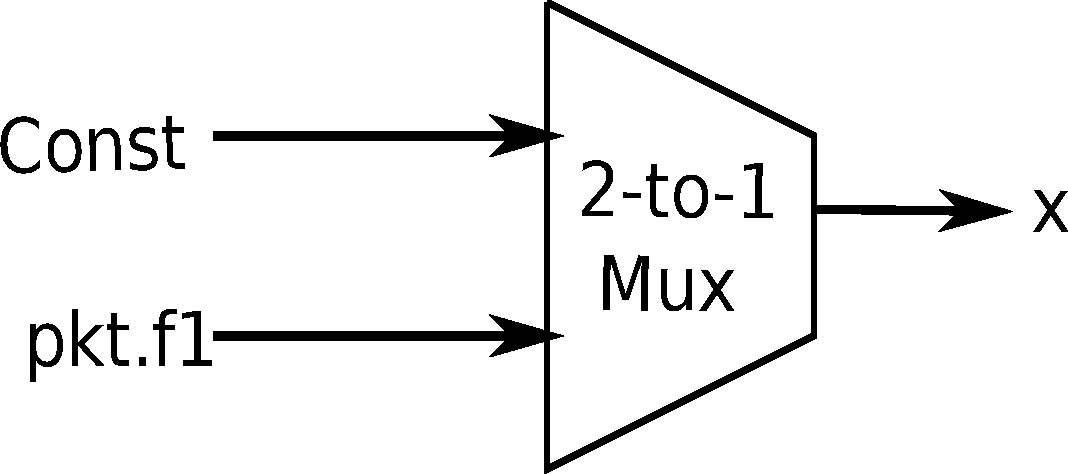
\includegraphics[width=0.2\textwidth]{domino_rw.pdf} & 176 \\
  \hline
  ReadAddWrite (RAW) & \centering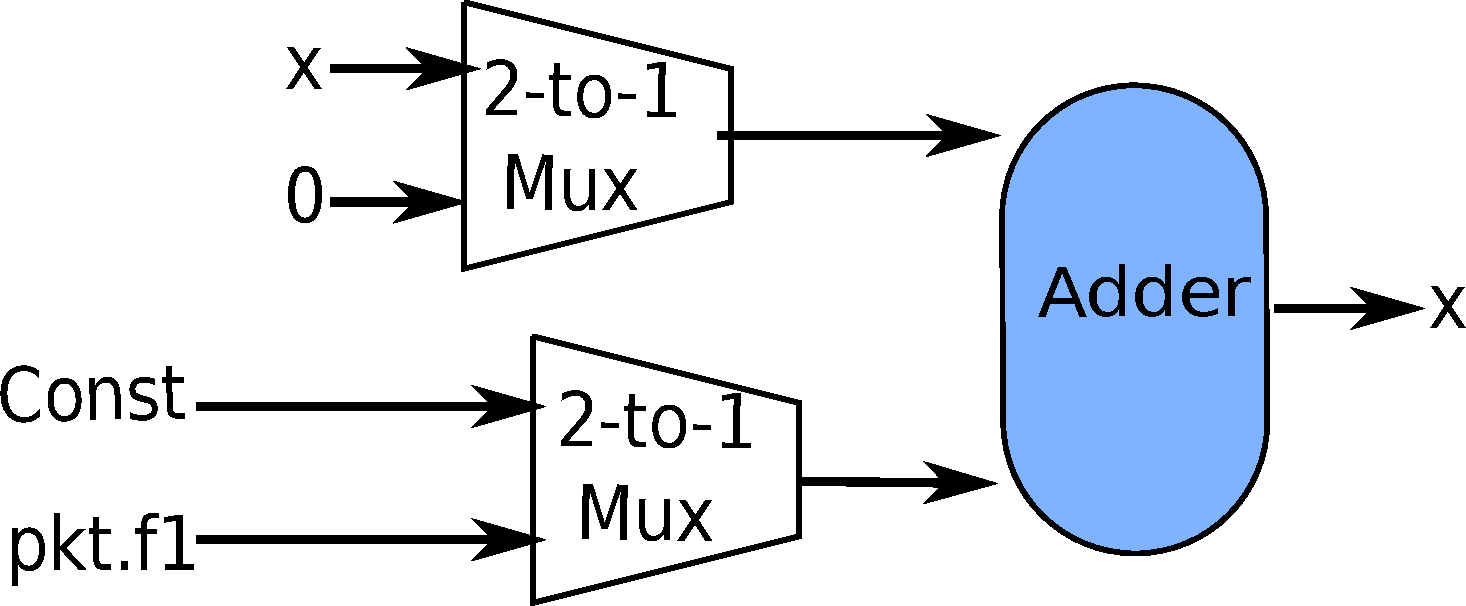
\includegraphics[width=0.25\textwidth]{domino_raw.pdf} & 316\\
  \hline
  \pbox{0.1\textwidth}
  {Predicated\\
  ReadAddWrite (PRAW)} & \centering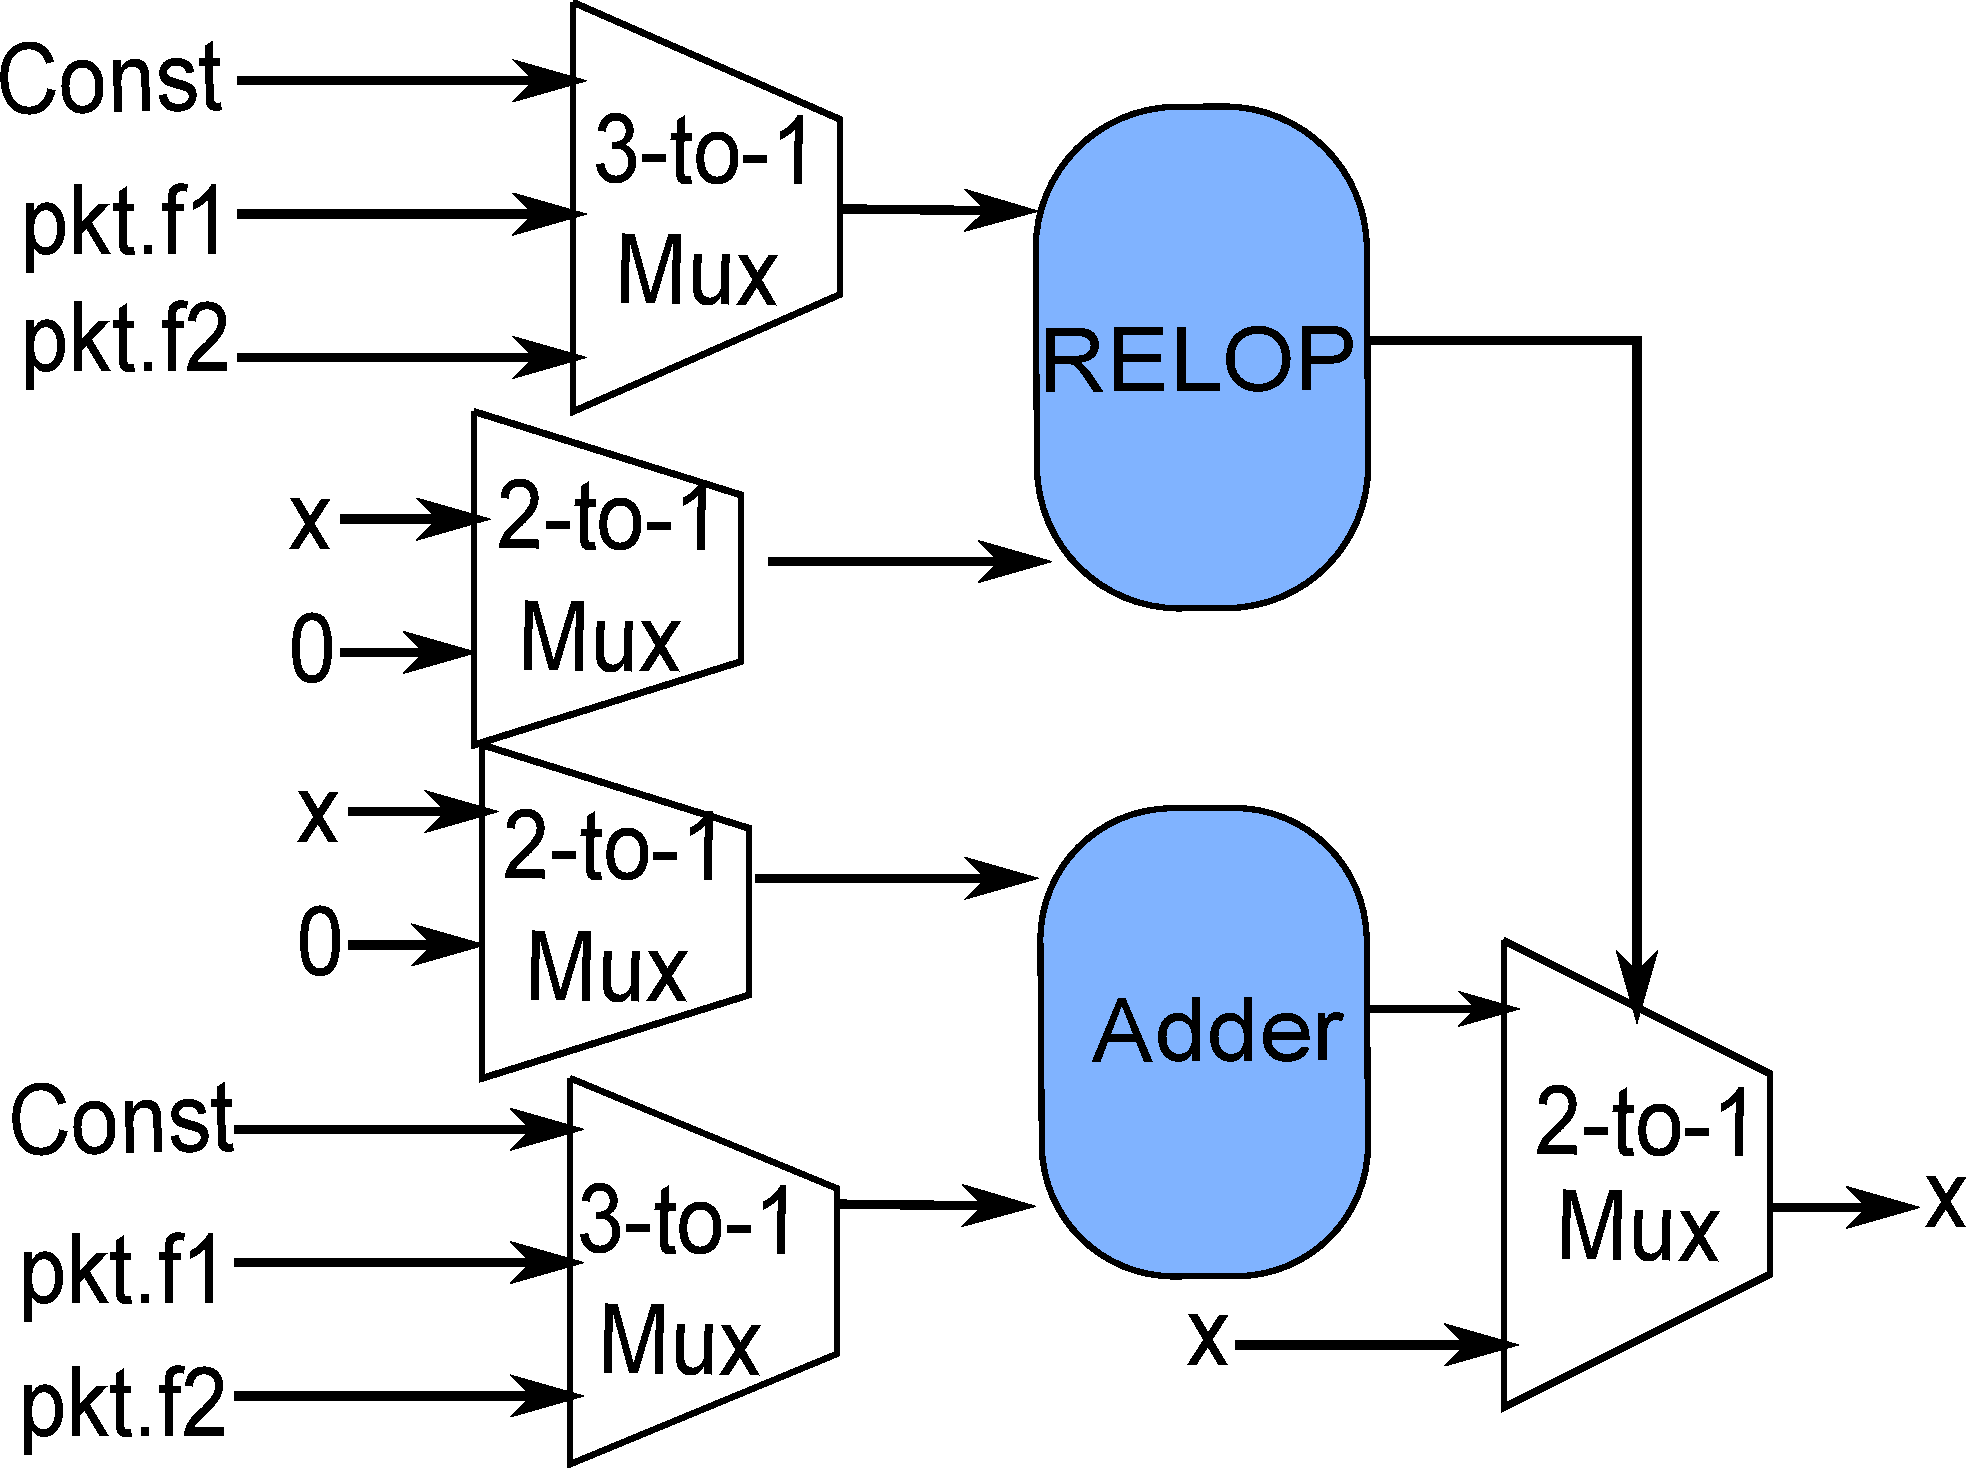
\includegraphics[width=0.3\textwidth]{domino_pred_raw.pdf}  & 393 \\
  \hline
  \end{tabular}
\end{scriptsize}
\caption{An atom's minimum critical-path delay increases with circuit depth.
Mux is a multiplexer. RELOP is a relational operation (>, <, ==, !=). {\tt x}
is a state variable. {\tt pkt.f1} and {\tt pkt.f2} are packet fields. {\tt
Const} is a constant operand.}
\label{tab:circuits}
\end{table}

\medskip
\noindent
\textbf{Compilers can be used to design instruction sets.}
Designing an instruction set for a programmable substrate is a chicken-and-egg
problem: the choice of instructions determines which algorithms can execute on
that target, while the choice of algorithms dictates what instructions are
required in the target. Indeed, other programmable substrates (GPUs, CPUs,
DSPs) go through an iterative process to design a good instruction set.

 A compiler can aid this process. To show how, we describe how we
designed the stateful atoms in Table~\ref{tab:templates}. We pick a data-plane
algorithm, partially execute the \pktlanguage compiler to generate a codelet pipeline,
inspect the stateful codelets, and create an atom that expresses
all the computations required by the stateful codelets. We check that an atom
can express all these computations by fully executing the compiler on the
data-plane algorithm with that atom as the target. We then move on to the next
algorithm, extending our atom through a process of trial-and-error to capture
more computations, and using the compiler to verify our intuitions on extending
atoms. In the process,  we generate a hierarchy of atoms, each of which works
for a subset of algorithms.

Our atom design process is manual and ad hoc at this point, but it already
shows how  a compiler can aid in instruction-set design for programmable
switches. Using the same iterative approach involving a compiler, we anticipate
the atoms in \absmachine machines evolving as data-plane algorithms demand more
of the hardware.

%%\textbf{Compilation time:}
%%Compilation time is dominated by SKETCH's search procedure.  To speed up the
%%search, we limit SKETCH to search for constants (e.g., for addition) of size up
%%to 5 bits, given that the constants seen within stateful codelets in our
%%algorithms are small. Our longest compilation time is 10 seconds when CoDel
%%doesn't map to a \absmachine machine with the Pairs atom because SKETCH has to
%%rule out every configuration in its search space.  This time will increase if
%%we increase the bit width of constants that SKETCH has to search; however,
%%because the data-plane algorithms themselves are small, we don't expect
%%compilation times to be a concern.
